\documentclass[aspectratio=149,11pt]{beamer}
\usepackage{graphicx}
\usepackage{longtable}
\usepackage{wrapfig}
\usepackage{rotating}
\usepackage[normalem]{ulem}
\usepackage{amsmath}
\usepackage{amssymb}
\usepackage{capt-of}
\usepackage{hyperref}
\institute{Università di Siena}
\usepackage{localheader}
\usepackage{tikz}
\usepackage{booktabs}
\usepackage{setspace}
\usepackage{quoting}
\usepackage[italian]{babel}
\usepackage{fancybox}
\usetheme{default}
\author{Massimo D'Antoni}
\date{Anno accademico 2023-2024}
\title{La spesa sociale\newline e lo Stato assicuratore}
\subtitle{Scienza delle Finanze}
\hypersetup{
 pdfauthor={Massimo D'Antoni},
 pdftitle={La spesa sociale\newline e lo Stato assicuratore},
 pdflang={Italian}}
\begin{document}

\maketitle

\section{Spesa sociale}

\begin{frame}{Protazione sociale, sicurezza sociale, \emph{welfare state}}
I termini sono (quasi) sinonimi, si riferiscono alle spese per la protezione
dei cittadini dal rischio e dal bisogno
\vspace{-3mm}

\begin{columns}
\begin{column}[t]{0.4\columnwidth}
\begin{itemize}
\item Convenzionalmente si considera spesa sociale la spesa rivolta ai seguenti rischi/bisogni specifici:
\end{itemize}
\end{column}

\begin{column}[t]{.58\columnwidth}
\begin{itemize}
\item malattia
\item invalidità
\item vecchiaia
\item superstiti
\item famiglia/figli
\item disoccupazione
\item abitazione
\item esclusione sociale (indigenza)
\end{itemize}
\end{column}
\end{columns}
\end{frame}

\begin{frame}{Protazione sociale, sicurezza sociale, \emph{welfare state} /2}
\begin{itemize}
\item Spesa sociale, spesa assistenziale, assistenza sociale\ldots{}\\[0pt]
chiariamo i termini
\end{itemize}

\begin{center}
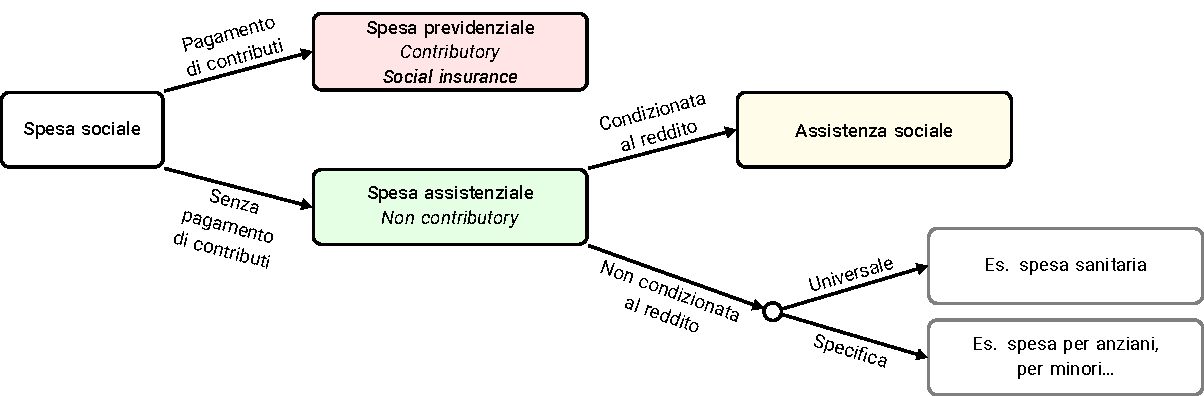
\includegraphics[width=\linewidth]{./figure/spesa-sociale-classificazione.pdf}
\end{center}

\begin{itemize}
\item L'ISTAT, nel presentare i dati sulla spesa sociale ("protezione sociale"), distingue tra:
\begin{itemize}
\item previdenza
\item sanità
\item assistenza (tutto il resto)
\end{itemize}
\end{itemize}
\end{frame}

\begin{frame}{La dimensione della spesa sociale pubblica (per funzioni)}
\begin{figure}[htbp]
\centering
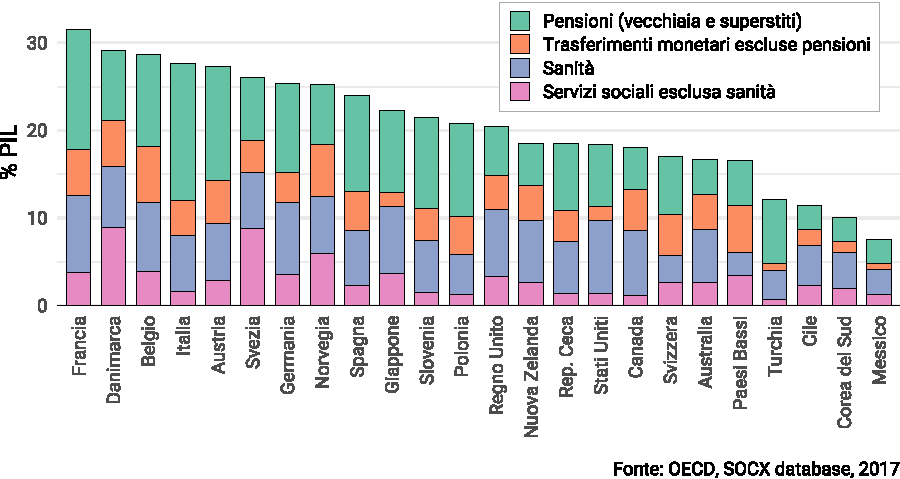
\includegraphics[width=.95\textwidth]{./figure/spesa-sociale-lorda-per-aree-principali-color.pdf}
\end{figure}
\end{frame}

\begin{frame}{La spesa sociale spiega buona parte dell'aumento della spesa pubblica}
\begin{figure}[htbp]
\centering
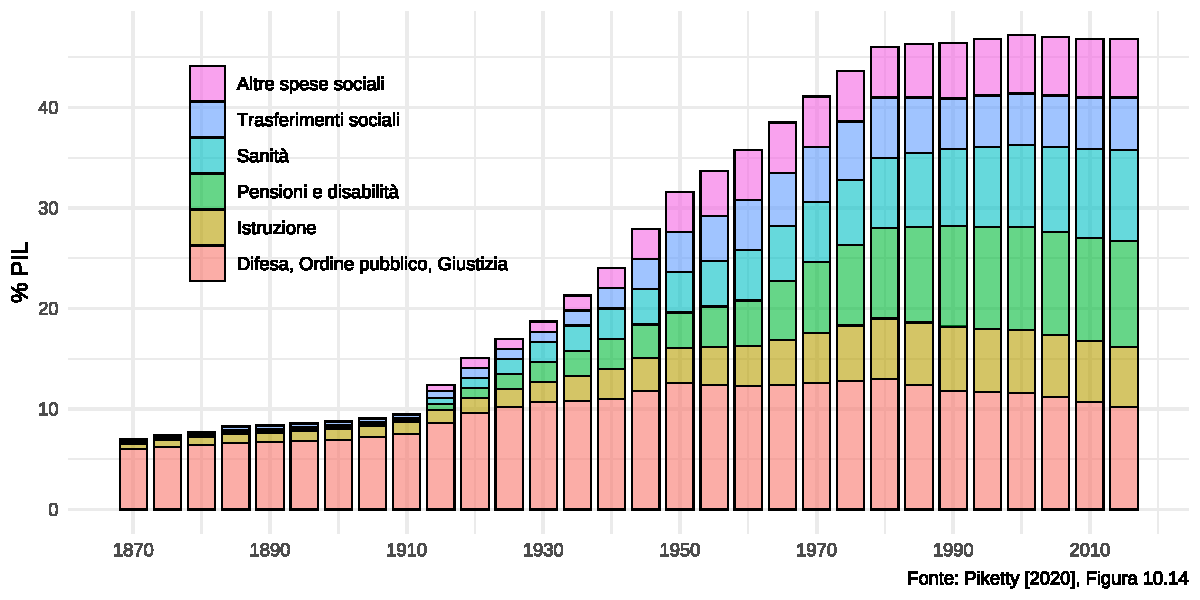
\includegraphics[width=.95\textwidth]{./figure/evoluzione-spesa-Piketty.pdf}
\end{figure}
\end{frame}


\begin{frame}{La spesa sociale può essere pubblica o privata}
\begin{figure}[htbp]
\centering
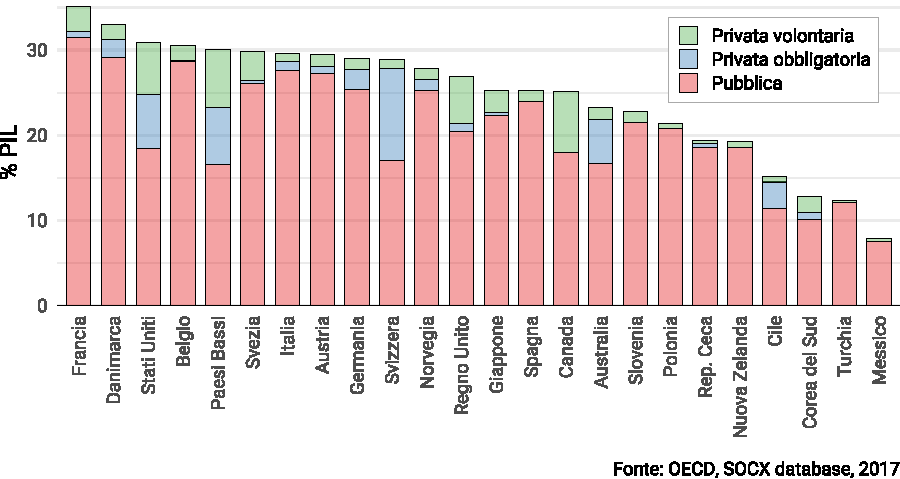
\includegraphics[width=.85\textwidth]{./figure/spesa-sociale-pubblica-privata-color.pdf}
\end{figure}

\small
\begin{itemize}
\item La spesa sociale può essere privata, purché in assenza di un corrispettivo
da parte del beneficiario e al di fuori di schemi assicurativi individuali
(es. assicurazione vita NON è spesa sociale).
\item Esempi di spesa sociale privata: erogazioni di enti caritativi, religiosi e
laici, associazioni di volontariato, che perseguono finalità mutualistiche o
di assistenza.
\end{itemize}
\end{frame}

\begin{frame}{Spesa sociale lorda e netta}
\begin{figure}[htbp]
\centering
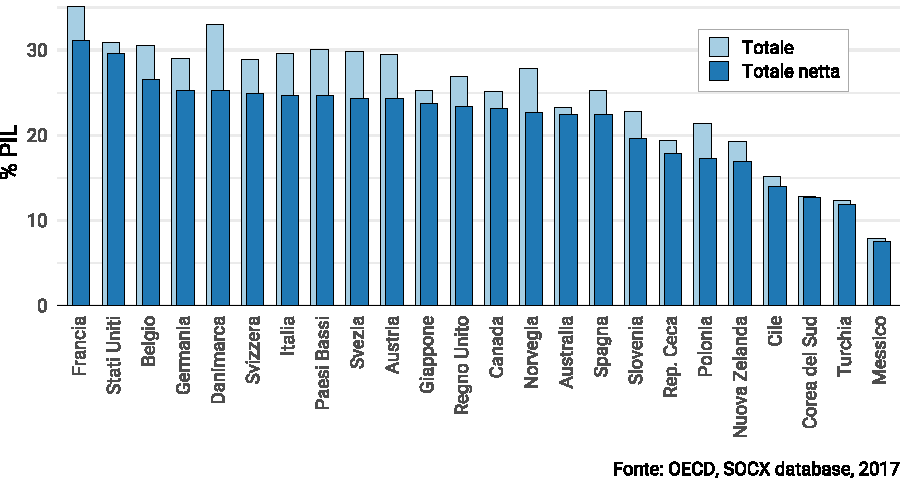
\includegraphics[width=.8\textwidth]{./figure/spesa-sociale-totale-lorda-netta-color.pdf}
\end{figure}

Per calcolare la spesa sociale netta correggiamo il dato sulla spesa sociale tenendo conto di:
\begin{itemize}
\item \emph{Tax expenditures}
\item Tassazione dei benefici (imposte dirette e indirette)
\end{itemize}
\end{frame}

\begin{frame}{I soggetti della protezione sociale in Italia}
\begin{itemize}
\item Il \alert{Servizio sanitario nazionale (SSN)} fornisce cure sanitarie a tutti i
cittadini. Finanziato con fiscalità generale e compartecipazione (\emph{ticket})
\item L'\alert{INPS}, Istituto Nazionale della Previdenza sociale, eroga prestazioni
previdenziali (pensioni IVS, indennità di disoccupazione e maternità) e
assistenziali (l’assegno sociale, l’assegno per il nucleo familiare,
l’assegno di accompagnamento, la pensione e il reddito di cittadinanza)
\item L'\alert{INAIL}, Istituto Nazionale per l’Assicurazione contro gli Infortuni sul
Lavoro, gestisce il sistema di assicurazione contro gli infortuni, le morti
sul lavoro e le malattie professionali.
\item I \alert{Comuni} servizi sociali e servizi di assistenza domiciliare destinati a
famiglie (principalmente asili nido), minori, disabili, anziani e persone in
condizioni di marginalità e disagio (solo 1,5\% della spesa)
\end{itemize}
\end{frame}

\section{La fornitura pubblica di assicurazione}

\begin{frame}{Lo stato fornisce assicurazione}
\begin{itemize}
\item La spesa sociale ha una funzione sia \alert{distributiva} che \alert{assicurativa}, anche se non è sempre facile distinguere i due aspetti
\item La spesa sociale svolge una funzione assicurativa rispetto agli effetti dei
grandi \alert{rischi} dell'esistenza:
\begin{itemize}
\item Assicurazione sanitaria (→ rischio malattia)
\item Pensioni (→ rischio longevità)
\item Sussidi di disoccupazione (→ rischio perdita del lavoro)
\item Pensioni di invalidità (→ rischio incidente o malattia invalidante)
\end{itemize}
\item Tra individui avversi al rischio la condivisione di rischi indipendenti
attraverso un meccanismo assicurativo determina un mutuo vantaggio. In molti
casi i mercati forniscono gli strumenti per realizzare tale condivisione del
rischio
\begin{itemize}
\item Il I teorema fondamentale dell'economia del benessere si applica anche al
caso di incertezza. In questo caso l'efficienza è raggiunta in presenza di
mercati assicurativi completi
\end{itemize}
\end{itemize}
\end{frame}

\begin{frame}{Perché non c'è assicurazione privata?}
\begin{itemize}
\item Per molti dei rischi collegati ai programmi di spesa sociale, non
esiste la possibilità di assicurarsi sul mercato
\begin{itemize}
\item in nessun paese del mondo le assicurazioni sanitarie private coprono
l'intera popolazione;
\item non esiste la possibilità di acquistare rendite per la vecchiaia
perfettamente indicizzate all'inflazione;
\item non esistono polizze private che assicurino l'individuo contro la perdita
di lavoro per vicende macroeconomiche;
\item in un contesto parzialmente diverso, i mercati del credito non permettono
a un giovane di finanziare tutto il corso formativo dando a esclusiva
garanzia i suoi redditi futuri.
\end{itemize}
I mercati privati per certi rischi semplicemente non esistono
\item Qual è in questo caso la natura del \alert{fallimento del mercato}?
\end{itemize}
\end{frame}

\begin{frame}{La convenienza ad assicurarsi}
\begin{itemize}
\item Supponiamo che vi siano \(n\) individui, ciascuno dei quali incorre nel
rischio di una perdita \(10.000\) con uguale probabilità \(\pi=0,1\)
\item Nel caso in cui uno o più individui subiscano una perdita, questa viene
suddivisa tra tutti i membri della collettività.
\item Invece di sostenere una perdita \(10.000\) con probabilità \(\pi\), ciascuno
avrà una perdita \(10.000\times k/n\), dove \(k\) è il numero di
individui che subiscono la perdita.
\item La convenienza del meccanismo assicurativo si basa sul fatto che, con \(n\)
elevato, \alert{se i rischi sono indipendenti}, il valore di \(k/n\) tende a non
scostarsi dalla probabilità della perdita \(\pi\) (\emph{legge debole dei grandi
numeri})
\end{itemize}
\end{frame}

\begin{frame}{La perdita attesa quando il rischio è condiviso}
\begin{columns}
\begin{column}{.4\columnwidth}
\small
\begin{itemize}
\item Per il singolo individuo la perdita è 10.000 con probabilità 1\%;
\item Se \(n=2\), se i rischi sono \alert{indipendenti}, la perdita è 5.000 con
probabilità 18\%, 10.000 con probabilità 1\%;
\item In generale, la probabilità che \(k\) su \(n\) individui subiscano la perdita, e
quindi ciascuno paghi \(k/n\times 10.000\), è pari a:
\begin{equation*}
  \frac{n!}{k!(n-k)!}\, \pi^k(1-\pi)^{n-k}.
\end{equation*}
\end{itemize}
\end{column}
\begin{column}{.6\columnwidth}
\begin{figure}[htbp]
\centering
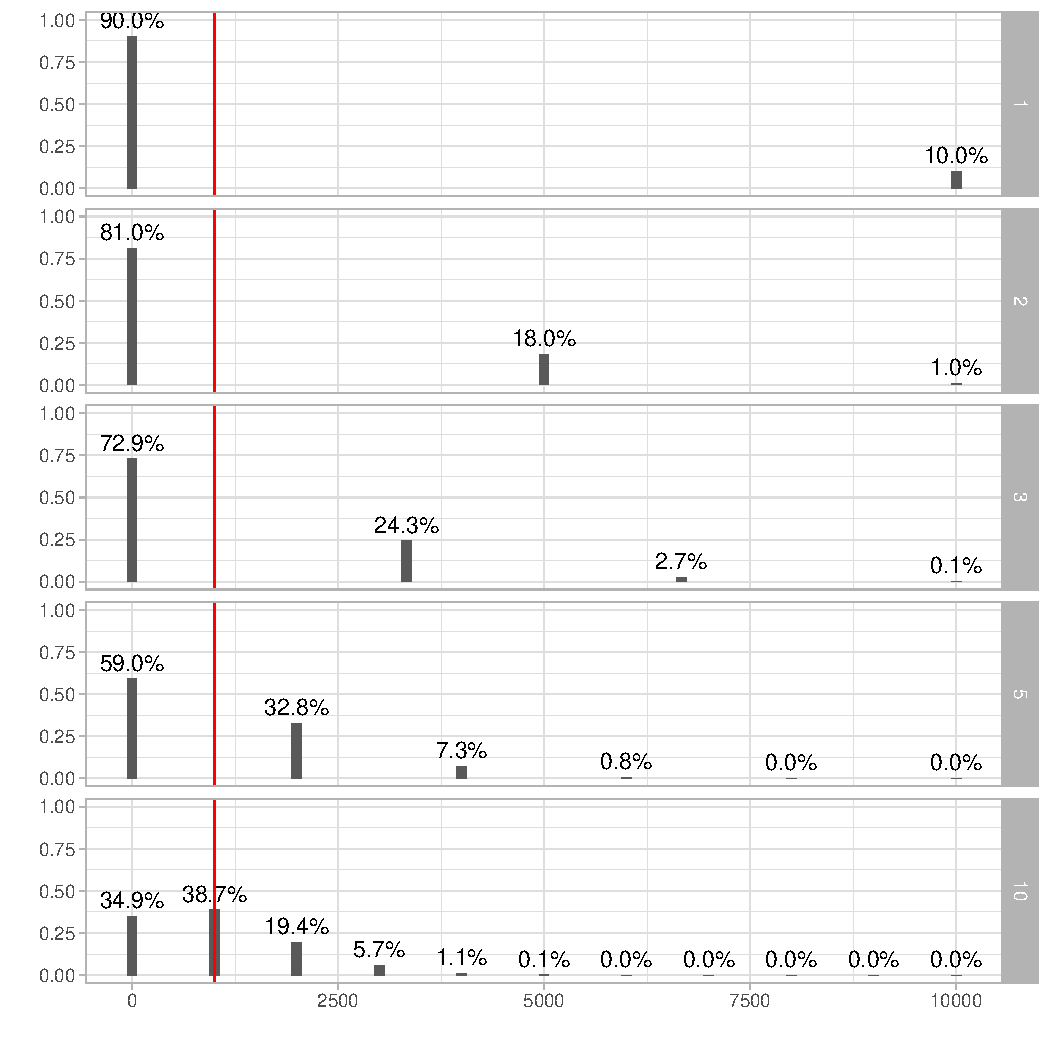
\includegraphics[width=\textwidth]{./figure/distribuzione-perdite.pdf}
\end{figure}
\end{column}
\end{columns}
\end{frame}

\begin{frame}{La perdita attesa quando il rischio è condiviso /2}
\begin{columns}
\begin{column}{.4\columnwidth}
\small
\begin{itemize}
\item All'aumentare del numero di individui che
condividono il rischio, la probabilità che la perdita media sopportata da
ciascuno si discosti dal valore atteso \(\pi \times 10.000 = 1.000\) si
riduce progressivamente e tende a zero.
\item Ad es. se \(n=1000\), la perdita media sarà con probabilità del 99\% compresa
tra 750 e 1.250.
\item Questo risultato è noto come \alert{legge debole dei grandi numeri} (\emph{la media
campionaria converge in probabilità al valore atteso delle variabili}).
\end{itemize}
\end{column}
\begin{column}{.6\columnwidth}
\begin{figure}[htbp]
\centering
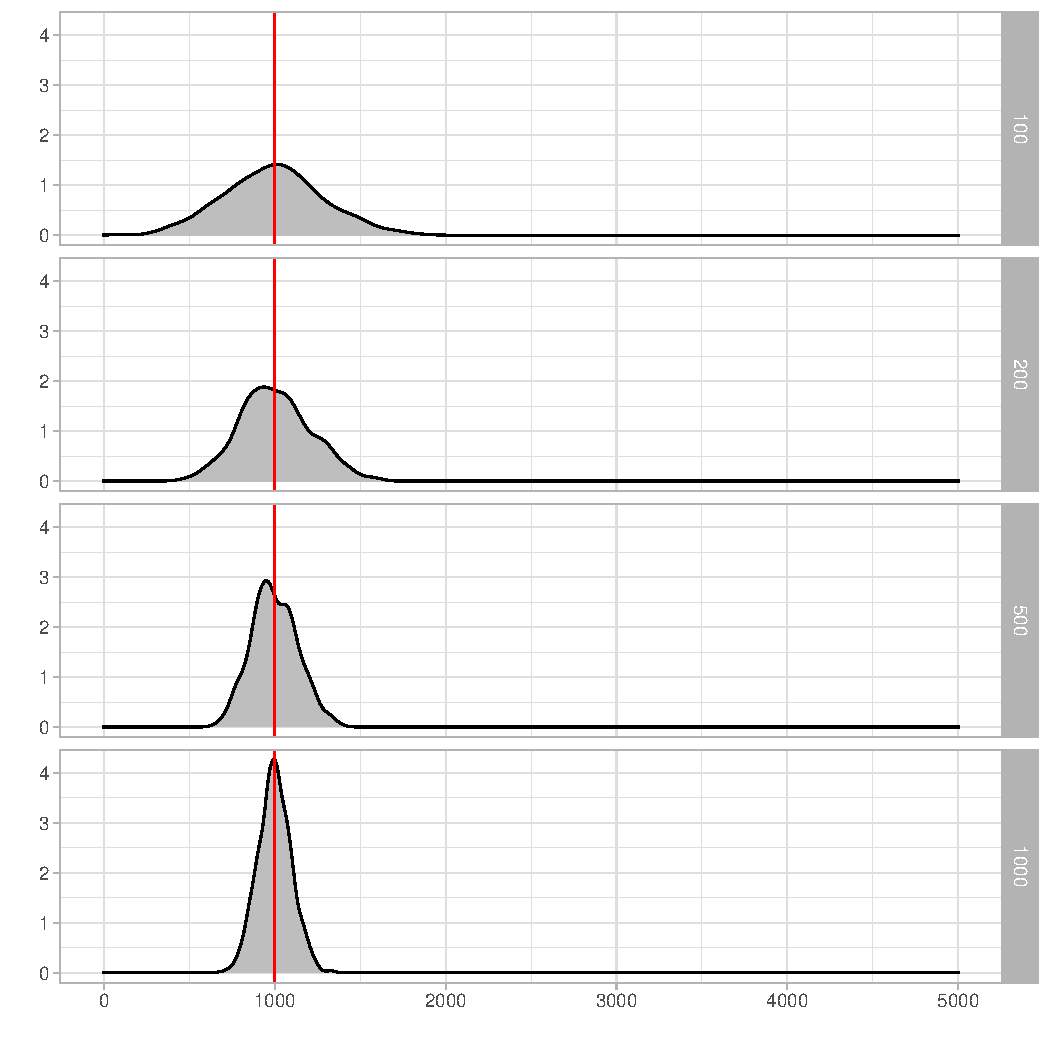
\includegraphics[width=\textwidth]{./figure/distribuzione-perdite-2.pdf}
\end{figure}
\end{column}
\end{columns}
\end{frame}


\begin{frame}{La varianza con rischi indipendenti e con rischi correlati}
\begin{itemize}
\item Lo stesso concetto si può esprimere considerando la varianza. Indicando con
\(L\) la perdita, per il singolo essa è pari a:
\begin{equation*}
  \text{var}[X_i]=\pi(L-\pi L)^2+(1-\pi)(0-\pi L)^2 =\pi(1-\pi)L^2.
\end{equation*}
mentre con due individui che condividono il rischio:
\begin{equation*}
\text{var}[\bar{X}] = \pi^2(L-\pi L)^2+2\pi(1-\pi)\left(L/2-\pi L\right)^2
+(1-\pi)^2(0-\pi L)^2=\frac{\pi(1-\pi)L^2}{2}.
\end{equation*}
\item Con \(n\) individui:
\begin{equation*}
  \text{var}\left[\frac{\sum_iX_i}{n}\right]
  =\frac{1}{n^2}\text{var}\left[\sum_iX_i\right]
  =\frac{1}{n^2}\sum_i\text{var}[X_i]=\frac{\pi(1-\pi)L^2}{n}.
\end{equation*}
\item Se i rischi sono correlati (cioè \(\text{cov}\not=0\)), la formula diventa
\begin{equation*}
\text{var}\left[\frac{\sum_iX_i}{n}\right]
=(1+\rho_{ij}(n-1))\frac{\pi(1-\pi)L^2}{n};
\end{equation*}
dove \(\rho_{ij}\) è il coefficiente di correlazione tra \(X_i\) e \(X_j\).
\end{itemize}
\end{frame}

\begin{frame}{La convenienza ad assicurarsi}
\begin{itemize}
\item Un individuo avverso al rischio trova sempre conveniente stipulare una polizza ad un
premio pari al risarcimento atteso
\begin{itemize}
\item Esempio: la prospettiva di un danno di 1000€ con probabilità 20\% comporta, per
un individuo avverso al rischio, un costo equivalente \alert{maggiore} di 200€
(= \(1000\times 0,2\))
\item Un premio pari al danno atteso è detto \alert{equo in senso attuariale}
\end{itemize}
\item Un assicuratore che assicura un numero elevato di individui con rischi
indipendenti è in grado di ridurre fino a eliminare la variabilità
nell'esborso medio, e dunque può offrire un premio equo in senso attuariale
senza incorrere in perdite
\item In presenza di un premio attuarialmente equo è conveniente per l'individuo
assicurarsi in modo completo
\end{itemize}
\end{frame}

\begin{frame}{L'avversione al rischio}
\begin{itemize}
\item Possiamo rappresentare l'avversione al rischio con il consueto strumento
delle curve di indifferenza, interpretando i due "beni" \(y_1\) e \(y_2\) come
il reddito (consumo) in due stati: nello stato 1 non si verifica il danno
(reddito \(y_1=y\)), nello stato 2 si verifica il danno (reddito \(y_2=y-L\))
\end{itemize}
\begin{columns}
\begin{column}{.5\columnwidth}
\begin{itemize}
\item Considerando l'utilità attesa, se la probabilità del verificarsi del
danno è \(\pi\), una curva di indifferenza è definita da: \((1-\pi)u(y_1)+\pi
  u(y_2)=\bar u\)
\item L'inclinazione è:
$$ -\frac{1-\pi}{\pi}\frac{u'(y_2)}{u'(y_2)} $$
\item Sulla
bisettrice (\(y_1=y_2\)) l'inclinazione si riduce a: $$ -\frac{1-\pi}{\pi} $$
\end{itemize}
\end{column}
\begin{column}{.5\columnwidth}
\begin{center}
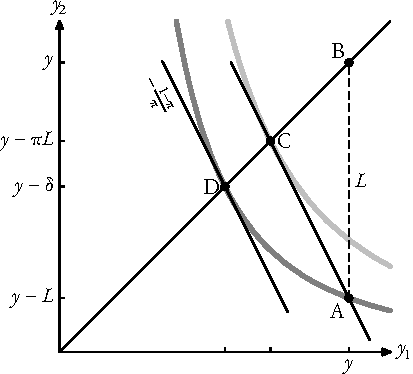
\includegraphics[width=.9\textwidth]{./figure/rischio-1.pdf}
\end{center}
\end{column}
\end{columns}
\end{frame}

\begin{frame}{L'avversione al rischio /2}
\begin{columns}
\begin{column}{.5\columnwidth}
\begin{itemize}
\item Lungo la retta passante per A e C il \alert{reddito atteso} \((1-\pi) y_1+\pi y_2\)
è costante e pari a \(y-\pi L\).
\item Nel punto C il reddito è pari a \(y-\pi L\) in entrambi gli stati.
\item Il punto D individua l'\alert{equivalente certo} \(\delta\), la perdita certa che
l'individuo considera equivalente alla perdita incerta \(L\) subita con
probabilità \(\pi\).
\item La differenza tra equivalente certo \(\delta\) è perdita attesa \(\pi L\) è
detta \alert{premio per il rischio}.
\end{itemize}
\end{column}

\begin{column}{.5\columnwidth}
\begin{center}
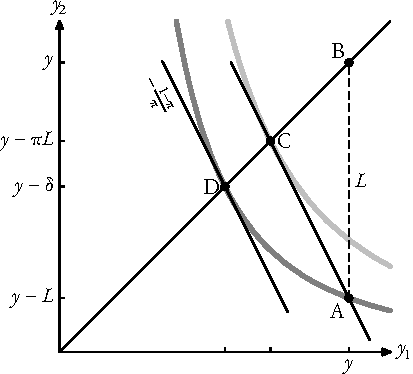
\includegraphics[width=.9\textwidth]{./figure/rischio-1.pdf}
\end{center}
\end{column}
\end{columns}
\end{frame}


\begin{frame}{L'avversione al rischio /3}
\begin{columns}
\begin{column}{.5\columnwidth}
Possiamo definire l'avversione al rischio equivalentemente in uno dei seguenti modi:
\begin{itemize}
\item l’utilità associata al rischio di subire una perdita \(L\) con probabilità
\(\pi\) è inferiore all’utilità associata a una perdita certa di ammontare
\(\pi L\);
\item la funzione \(u\) è concava (o anche: le curve di indifferenza sono convesse);
\item l'equivalente certo \(\delta\) è superiore alla perdita attesa \(\pi L\);
\item il premio per il rischio \(\delta-\pi L\) è (strettamente) positivo.
\end{itemize}
\end{column}

\begin{column}{.5\columnwidth}
\begin{block}{}
\small
\begin{itemize}
\item Un maggiore avversione al rischio corrisponde a una maggiore convessità
delle curve di indifferenza
\end{itemize}

\begin{center}
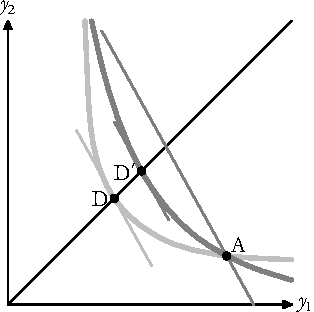
\includegraphics[width=.9\textwidth]{./figure/rischio-5.pdf}
\end{center}
\end{block}
\end{column}
\end{columns}
\end{frame}


\begin{frame}{L'avversione al rischio /3}
\begin{columns}
\begin{column}{.5\columnwidth}
\begin{itemize}
\item Se un individuo è avverso al rischio, troverà vantaggioso acquistare
copertura assicurativa completa quando questa viene offerta a un prezzo
\(q=\pi L\) (prezzo \alert{attuarialmente equo}).
\item Se invece il premio è superiore al livello attuarialmente equo (\(q>\pi L\))?
In questo caso ottimale acquistare copertura assicurativa non completa o non
assicurarsi.
\end{itemize}
\end{column}

\begin{column}{.5\columnwidth}
\begin{center}
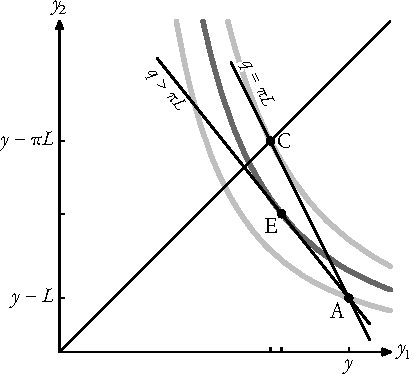
\includegraphics[width=.9\textwidth]{./figure/rischio-3.pdf}
\end{center}
\end{column}
\end{columns}
\end{frame}


\begin{frame}{I fallimenti dei mercati assicurativi}
Se assicurarsi è sempre vantaggioso per un individuo avverso al rischio, perché alcuni rischi non trovano copertura nei mercati assicurativi?

\begin{itemize}
\item \alert{Selezione avversa}: gli individui hanno una diversa rischiosità e il
livello di rischio individuale è noto all'assicurato ma non all'assicuratore\\[0pt]
→ i bassi rischi sceglieranno di non assicurarsi, il mercato può scomparire
\item \alert{Azzardo morale}: l'assicuratore non può osservare/controllare il
comportamento dell'assicurato
→ non c'è convenienza ad assicurarsi
\item \alert{Correlazione dei rischi}: se i rischi non sono indipendenti, non è
possibile ridurre la varianza media. In caso di evento avverso
l'assicuratore rischia la bancarotta
\item \alert{Costi di transazione}: se le circostanze che definiscono l'evento incerto o
la copertura del relativo rischio non sono ben specificabili in anticipo
\end{itemize}
\end{frame}

\section{La selezione avversa:\newline costi e possibili rimedi}

\begin{frame}{Eterogeneità dei rischi individuali}
\begin{itemize}
\item Gli individui hanno diverso danno/spesa perché la spesa è incerta (il che
rende vantaggiosa l'assicurazione), ma hanno anche diverso rischio di
incorrere nel danno/spesa
\item Se tale eterogeneità dipende da variabili osservabili, è possibile offrire a
ciascuno assicurazione con un premio pari al rischio individuale
\begin{itemize}
\item È accettabile che un individuo con una probabilità diversa di ammalarsi
debba sostenere costi più elevati?
\end{itemize}
\item Se non si possono applicare premi diversi (ad es. perché la fonte
dell'eterogeneità non è osservabile) si dovrà applicare un premio uniforme a
individui con rischi diversi
\item Ciò implica che per alcuni individui il premio potrebbe essere
significativamente più elevato del costo atteso: può aver luogo la
cosiddetta \alert{selezione avversa}
\end{itemize}
\end{frame}

\begin{frame}{Selezione avversa/1}
\begin{itemize}
\item \(\pi_i\) = probabilità di subire un danno \(L=1000\)
\item premio per il rischio \(a\pi_iL\), per cui massima disponibilità a pagare per
l'assicurazione è \((1+a)\pi_iL\) (assumiamo \(a=0,2\))
\end{itemize}

\begin{center}
\begin{tabular}{lccccl}
  \toprule
  $i$&rischio: $\pi_i$&perdita attesa& max premio\\
  \midrule
  1 & 0,2 &200 & 240 \\
  2 & 0,3 &300 & 360 \\
  3 & 0,4 &400 & 480 \\
  4 & 0,5 &500 & 600 \\
  \bottomrule
\end{tabular}  
\end{center}

\begin{itemize}
\item Se non posso distinguere i vari "tipi", quale premio applicherò?
\end{itemize}
\end{frame}

\begin{frame}{Selezione avversa/2}
\begin{itemize}
\item Consideriamo differenze più piccole nei rischi e maggiore avversione al rischio (\(a=0,34\))
\end{itemize}

\begin{center}
\begin{tabular}{lccccl}
  \toprule
  $i$&rischio: $\pi_i$&perdita attesa& max premio\\
  \midrule
  1 & 0,25 &250 & 335 \\
  2 & 0,3 &300 & 402 \\
  3 & 0,35 &350 & 469 \\
  4 & 0,4 &400 & 536 \\
  \bottomrule
\end{tabular}
\end{center}

\begin{itemize}
\item Tra gli individui vi sono \alert{sussidi incrociati}: chi ha rischio più basso finanzia l'assicurazione per chi ha rischio più alto

\item Possibile proporre polizze differenziate che attraggano in modo selettivo i
soli individui a basso rischio
\begin{itemize}
\item Se questo non è possibile sulla base di caratteristiche osservabili (es. età
o altro) possibile offrire diverso livello di copertura o diversi servizi
accessori
\end{itemize}
\end{itemize}
\end{frame}

\begin{frame}{Selezione avversa/3}
\begin{itemize}
\item Differenze più marcate, con presenza di individui che hanno un rischio di subire il danno vicino a 1 (100\%). Il premio per il rischio si avvicina a zero man mano che la probabilità del danno si avvicina a 1.
\end{itemize}

\begin{center}
\begin{tabular}{lccccl}
  \toprule
  $i$&rischio: $\pi_i$&perdita attesa & max premio\\
  \midrule
  1 & 0,4 &400 & 500 \\
  2 & 0,6 &600 & 720 \\
  3 & 0,8 &800 & 880 \\
  4 & 1,0 &1000&1000 \\
  \bottomrule
\end{tabular}
\end{center}
\end{frame}

\begin{frame}{Se posso differenziare i premi o le condizioni assicurative}
\begin{itemize}
\item La presenza di sussidi incrociati è incompatibile con la concorrenza, dal
momento che un assicuratore potrebbe selezionare i migliori rischi,
effettuando una "scrematura" (\emph{cream-skimming})
\item Questo è possibile se il livello di rischio dell'individuo è osservabile ed
è consentito discriminare i premi
\item N.B. l'assicuratore potrebbe comunque realizzare una selezione in modo
indiretto, ad esempio offrendo polizze caratterizzate da copertura parziale
che risultano attraenti solo per i bassi rischi
\item Pertanto: in concorrenza, i contratti \emph{pooling} non sono praticabili. Ma
questo è un problema? Si pone una questione di equità o di efficienza?
\begin{itemize}
\item Esempio: negli Stati Uniti Blue Cross/BLue Shield costretta dalla
concorrenza delle assicurazioni for profit a passare da \emph{community rating}
a \emph{experience rating}
\end{itemize}
\end{itemize}
\end{frame}

\begin{frame}{Soluzioni possibili al problema della selezione avversa}
\begin{itemize}
\item Assicurazione uniforme obbligatoria 

\begin{itemize}
\item Non è un miglioramento paretiano: per gli individui a basso
rischio l'acquisto di assicurazione comporta una riduzione dell'utilità

\item È un miglioramento di efficienza \emph{potenziale}: il guadagno di chi guadagna
eccede la perdita di chi perde
\end{itemize}

\item Sussidi all'acquisto di assicurazione

\begin{itemize}
\item Si incentiva l'acquisto anche da parte di individui a basso rischio

\item È un miglioramento paretiano?
\begin{itemize}
\item Dal momento che il sussidio deve essere finanziato, dipende dalla
distribuzione del carico fiscale
\end{itemize}
\end{itemize}
\end{itemize}
\end{frame}

\begin{frame}{La differenziazione dei premi è efficiente/equa?}
\begin{itemize}
\item È efficiente che ciascuno paghi un premio commisurato al rischio
\item Applicare un premio comune a individui con rischio diverso equivale a
redistribuire a favore dell'individuo con rischio più alto
\item È giusto che gli individui con diverso rischio paghino premi diversi? Non
sarebbe più equo applicare un premio uniforme?
\begin{itemize}
\item Se consideriamo che un individuo non sia responsabile del proprio maggiore
rischio e che la collettività deve farsi carico della sua maggiore
"sfortuna"\ldots{}
\end{itemize}
\item Come cambia la nostra risposta se consideriamo un orizzonte temporale più
lungo e la necessità di rinnovare le condizioni del contratto assicurativo?
\begin{itemize}
\item Il verificarsi dell'evento avverso (es. malattia) potrebbe
determinare un aumento della rischiosità attribuita all'individuo
dall'assicuratore (\emph{reclassification risk})
\end{itemize}
\end{itemize}
\end{frame}

\begin{frame}{La differenziazione dei rischi nel tempo e il rischio di riclassificazione}
\small
\begin{itemize}
\item Supponiamo che l'individuo abbia il 20\% di probabilità di ammalarsi in
ciascun periodo. Il costo della malattia è 1.000€
\item Tuttavia, la probabilità \alert{condizionata} di ammalarsi nel secondo periodo è
diversa a seconda che l'individuo si sia ammalato o no nel primo periodo:
\begin{itemize}
\item probabilità di riammalarsi se si è già ammalato: 40\%
\item probabilità di riammalarsi se non si è ammalato: 15\%
\item Dunque, la probabilità incondizionata di ammalarsi nel secondo periodo è:\\[0pt]
20\% \texttimes{} 40\% + 80\% \texttimes{} 15\% = 20\%
\end{itemize}
\item Stipulando all'inizio un contratto per due periodi pagherebbe un premio di
200€ + 200€ = 400€
\item Assicurandosi periodo per periodo, pagherà un premio di 200€ nel primo
periodo, mentre nel secondo periodo l'assicuratore potrà condizionare il
premio allo stato di salute osservato (\emph{experience rating}), dunque:
\begin{itemize}
\item un premio di 400€ se si è ammalato nel primo periodo
\item un premio di 150€ se non si è ammalato nel primo periodo
\end{itemize}
\item Il fatto che l'individuo soffra il rischio di pagare un premio più elevato
rappresenta un'\alert{inefficienza} (non ottiene piena copertura dal rischio)
\end{itemize}
\end{frame}

\begin{frame}{Riassumendo}
\begin{enumerate}
\item È ottimale assicurarsi completamente quando gli individui sono avversi al
rischio e il premio offerto è equo in senso attuariale
\item Quando la popolazione di assicurati è eterogenea, offrendo un contratto
uniforme (\emph{pooling}) si rischia la \emph{selezione avversa}
\item Anche in assenza di selezione avversa, la concorrenza porta alla
\emph{scrematura} con segmentazione tra alti e bassi rischi
\item Un mercato segmentato è efficiente \emph{ex post}, ma inefficiente \emph{ex ante}
perché espone al \emph{rischio di riclassificazione} e discontinuità della
copertura assicurativa
\item L'applicazione di premi uniformi indipendenti dal rischio individiale può
inoltre rispondere anche a un criterio di equità
\item Tuttavia, l'applicazione di premi uniformi a individui con rischio
differenziato può risultare incompatibile con la concorrenza
\end{enumerate}
\end{frame}

\begin{frame}{Perché nessuno offre contratti a lungo termine?}
\begin{itemize}
\item In astratto il problema della differenziazione dei premi sarebbe risolto da
un contratto a lungo termine con premio costante. Tuttavia:
\begin{itemize}
\item Portabilità geografica (la polizza deve mantenere validità a fronte di
spostamento dell'assicurato in un'area diversa)
\item Incompletezza contrattuale: non è possibile sapere in anticipo quali
trattamenti saranno disponibili in futuro. Il contratto dovrà quindi
essere rinegoziato e a quel punto l'assicuratore potrebbe escludere i
pazienti ad alto rischio
\end{itemize}
\item In alternativa, l'assicuratore potrebbe fornire un generico impegno a
coprire le spese sanitarie, assumendosi il rischio connesso all'evoluzione
della spesa sanitaria su un orizzonte lungo.
\begin{itemize}
\item Ma qual è il "valore" di un'assicurazione sanitaria tra vent'anni?
\end{itemize}
\item L'incapacità del mercato di risovere questo problema è una delle ragioni
principali per cui solo il pubblico è in grado di fornire ampia copertura
assicurativa rispetto al rischio di ammalarsi
\end{itemize}
\end{frame}

\begin{frame}{Il finanziamento delle cure sanitarie nelle economie avanzate/1}
\begin{figure}[htbp]
\centering
\includegraphics[width=\textwidth]{./figure/schemi-finanziamento-sanità.png}
\end{figure}
\end{frame}


\begin{frame}{Il finanziamento delle cure sanitarie nelle economie avanzate/2}
\begin{itemize}
\item Dove c’è scelta il pacchetto di servizi di base forniti è solitamente
definito dal governo
\item Spesso anche il livello del premio è fissato e non può essere modificato
\item Gli spazi per definire termini e contenuto del pacchetto sono regolati
\item Inoltre, generalmente abbiamo:
\begin{itemize}
\item divieto di rifiutare rinnovo
\item vincoli agli aumenti in caso di rinnovo
\end{itemize}
\item Meccanismi di "aggiustamento del rischio"
\begin{itemize}
\item Paesi Bassi, Germania e Svizzera: aggiustamento basato su età e sesso. In
Paesi Bassi anche regione e gruppo diagnostico, in Germania presenza di
patologie croniche
\item Germania: i fondi prelevano dagli assistiti contributi in proporzione al
reddito, che vengono redistribuiti in base alle caratteristiche degli
assistiti. Possibile offrire condizioni differenziate (es. premio più
basso in cambio di restrizioni sulla scelta dei fornitori o maggiore
compartecipazione ai costi). Perdite e guadagni dei fondi si traducono in
riduzioni/aumenti dei premi
\end{itemize}
\end{itemize}
\end{frame}

\begin{frame}{Spesa sanitaria pubblica e privata}
\begin{figure}[htbp]
\centering
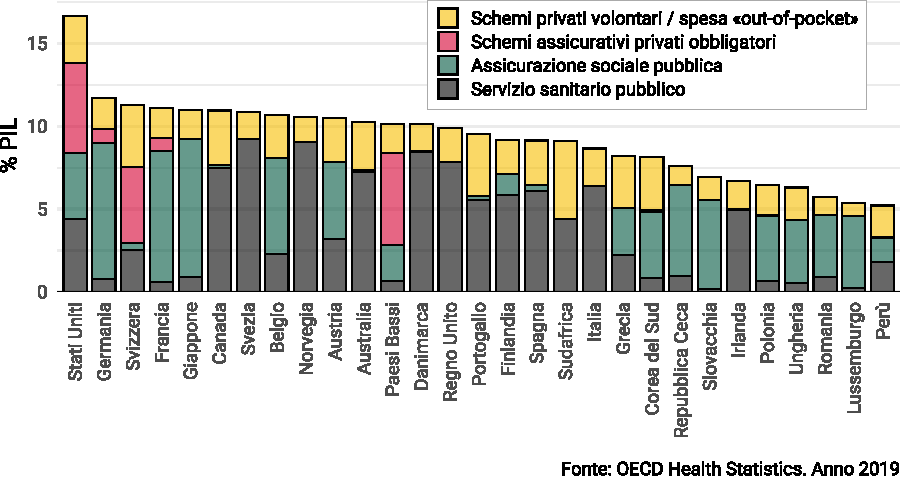
\includegraphics[width=.95\textwidth]{./figure/spesa-sanitaria-per-schema-color.pdf}
\end{figure}
\end{frame}

\section{Sistemi sanitari a confronto:\newline USA e Italia}

\begin{frame}{Il SSN italiano: Principi ispiratori e caratteristiche generali}
\begin{itemize}
\item Istituito nel 1977, a partire dal 1978, per superare il precedente sistema
mutualistico, frammentato (più di 100 enti mutualistici nel 1970) e con
limitazioni alla copertura (7\% popolazione non coperta)
\item Ispirato al National Health Service britannico del 1948, ma più decentrato
\item Principi
\begin{itemize}
\item Universalità del servizio
\item Gratuità al momento dell'erogazione
\item Ispirato a principi di solidarietà ed eguaglianza di accesso (inclusi gli
immigrati dal 1998: immigrati legali con pieni diritti, illegali accesso limitato)
\end{itemize}
\item Negli anni '90 progressiva devoluzione della responsabilità in campo
sanitario alla Regioni e conferimento di autonomia gestionale alle ASL e
ospedali (aziendalizzazione, modello dei "mercati interni")
\item Nel 1999 completamento della regionalizzazione della sanità (al livello
nazionale resta la fissazione di obiettivi generali e standard---i LEA,
Livelli essenziali di assistenza). Maggiore enfasi su cooperazione e
regolazione.
\item La regionalizzazione ha determinato una notevole varietà e differenziazione
dei livelli
\end{itemize}
\end{frame}
\begin{frame}{Differenze nei livelli di soddisfazione a livello regionale}
\begin{figure}[htbp]
\centering
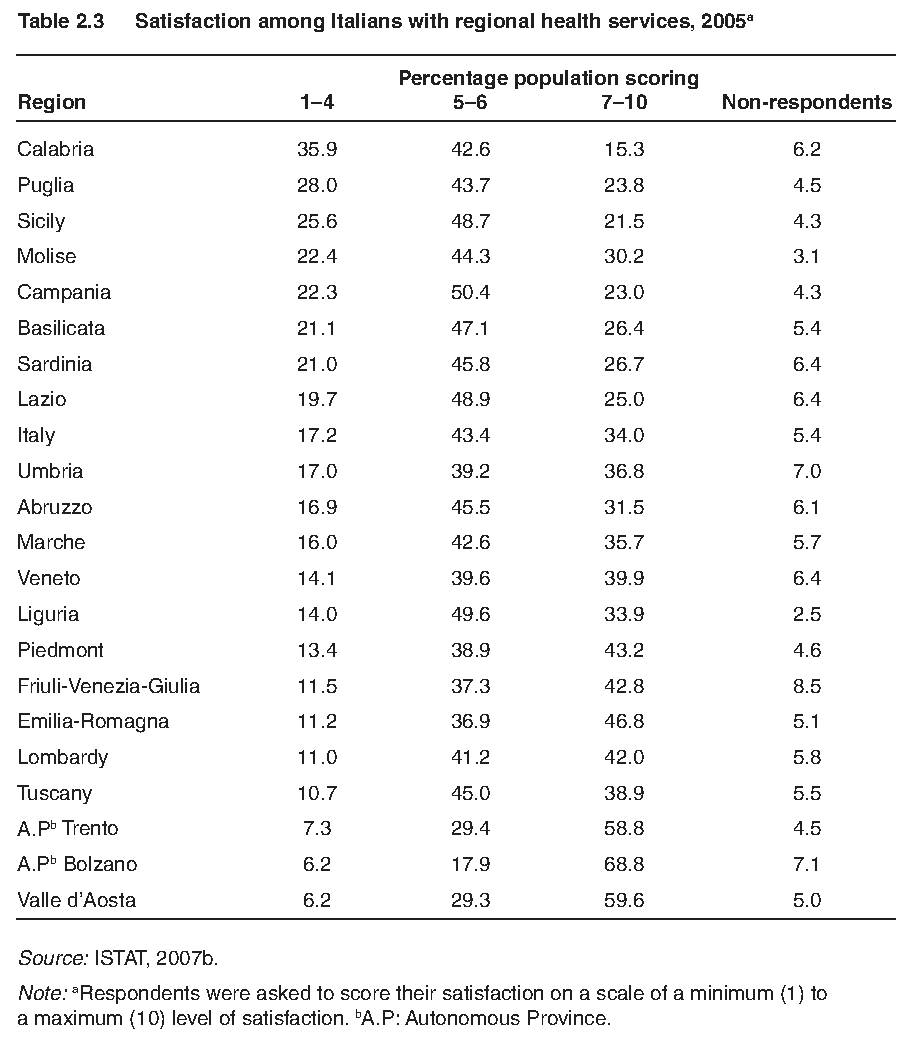
\includegraphics[height=7cm]{./figure/soddisfazione-sanita-italiana-regioni.pdf}
\end{figure}
\end{frame}

\begin{frame}{Il finanziamento è prevalentemente pubblico, ma\ldots{}}
\begin{itemize}
\item La spesa sanitaria pubblica è parte preponderante della spesa regionale
\item Finanziamento del bilancio regionale attraverso 
\begin{itemize}
\item \alert{IRAP}: un'imposta che grava sul valore aggiunto delle imprese
\item \alert{Addizionale regionale IRPEF}
\item \alert{Compartecipazione all'IVA} utilizzata per perequare le risorse, vista la
diversa distribuzione dell'IRAP --- la perequazione attraverso il Fondo di
solidarietà regionale è una questione politica rilevante, negoziata dalla
Conferenza Stato Regioni
\end{itemize}
(fino al 2000 esisteva il Fondo sanitario regionale)
\item Scarso ruolo delle assicurazioni sanitarie (5\%), che coprono co-pagamenti e
servizi non coperte dal SSN e ricorso ai privati
\item Ruolo non irrilevante della spesa \emph{out-of-pocket} (circa 20\%), che
comprende compartecipazione al costo (\emph{ticket})
\item N.B. Fino al 1998 finanziamento attraverso contributi sanitari, regressivi
\end{itemize}
\end{frame}

\begin{frame}{La fornitura dei servizi è mista, pubbica e privata}
\begin{itemize}
\item ASL con ruolo di supervisione e fornitura di servizi di prevenzione, igiene
ecc.
\item Medici e pediatri di base sono liberi professionisti a contratto,
remunerati su base capitaria
\item Ambulatori di diagnostica e altri servizi specialistici, forniti dalle ASL
oppure privati accreditati o sotto contratto con le ASL
\item Ospedali pubblici (circa 650) e privati accreditati (circa 550). I
principali sono \emph{aziende ospedaliere} dotate di autonomia (sottratte alla
direzione delle ASL)
\item Farmacie pubbliche (per lo più comunali, meno del 10\%) o private sotto
contratto
\end{itemize}
\end{frame}

\begin{frame}{La sanità USA prima della riforma Obama del 2010}
\begin{itemize}
\item Gli USA erano il solo grande paese industrializzato che non riusciva a
garantire una copertura assicurativa universale.
\item In parte anche ragioni ideologiche: percentuale consistente, tra il 40 e il
50\%, ritiene che la salute dei cittadini non sia una responsabilità dello
Stato

\item Copertura assicurativa nel 2006 (categorie non mutuamente esclusive):
\end{itemize}

\small
\begin{center}
\begin{tabular}{{lr}}
\hline
\alert{Private insurance} & \\[0pt]
Employment-based private insurance & 59.7\%\\[0pt]
Direct-purchase & 9.1\%\\[0pt]
Any private plan & 67.9\%\\[0pt]
\hline
\alert{Government insurance} & \\[0pt]
Medicare & 13.6\%\\[0pt]
Medicaid & 12.9\%\\[0pt]
Military health care & 3.6\%\\[0pt]
Any government plan & 27.0\%\\[0pt]
\hline
\alert{No insurance} & \\[0pt]
Not covered & 15.8\%\\[0pt]
\hline
\end{tabular}
\end{center}

\footnotesize Source: \href{http://www.census.gov/prod/2008pubs/p60-235.pdf}{US Census Bureau}
\end{frame}

\begin{frame}{L'Affordable Care Act ("Obamacare")}
\small
\begin{itemize}
\item Obiettivi della riforma del 2010: estendere la copertura assicurativa
rendendola accessibile, limitare la crescita della spesa
\item Introduzione di un (quasi)obbligo con penalizzazione fiscale a carico di
datori di lavoro e individui privi di assicuazione finanziaria (esclusioni
per reddito basso, motivi religiosi, immigrati irregolari, nativi)
\item Sussidi a piccole imprese e a individui a basso reddito
\item Creazione di "mercati" (\emph{exchanges}) gestiti dagli stati per consentire
l'acquisto di polizze a condizioni standardizzate (garanzia di servizi
essenziali)
\item Ampliamento della platea del programma Medicaid
\item Divieto e limitazione di pratiche che riducevano la copertura assicurativa:
\begin{itemize}
\item pre-existing conditions
\item tetti alla spesa annua o \emph{lifetime}
\item discriminazione dei premi (ora consentita entro limiti solo per età e
fumatori)
\end{itemize}
\item Divieto di rifiutare la polizza, di cancellarla unilateralmente o di
aumentare in modo irragionevole il premio
\end{itemize}
\end{frame}

\begin{frame}{Gli effetti della riforma}
\begin{figure}[htbp]
\centering
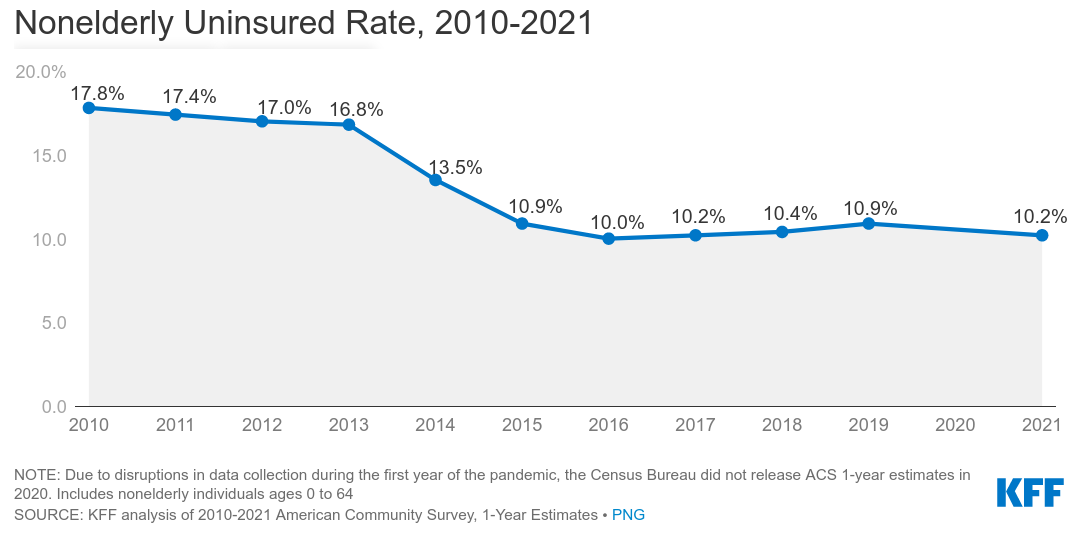
\includegraphics[height=5.5cm]{./figure/nonelderly-uninsured-rate.png}
\end{figure}

\begin{itemize}
\item Riduzione significativa del numero di non assicurati
\item Tuttavia:
\begin{itemize}
\item ancora una percentuale consistente non è coperta
\item resta notevole eterogeneità di trattamenti e condizioni
\end{itemize}
\end{itemize}
\end{frame}

\section{Assicurazione e incentivi}

\begin{frame}{Un argomento contro la fornitura di assicurazione: l'azzardo morale}
\begin{itemize}
\item Arrow (1963): «gli argomenti a favore dell'assicurazione sono
schiaccianti. Ne segue che il governo deve fornire assicurazione in tutti i
casi in cui, per qualche ragione, non si è creato un mercato assicurativo»
\item Controargomento: rischiamo di fornire assicurazione a un costo superiore
rispetto al beneficio, perché l'assicurazione spinge ad acquistare cure che
hanno un valore inferiore al costo.
\item \alert{Azzardo morale}: l'assicurazione modifica il comportamento degli
assicurati, induce scelte inefficienti.
\end{itemize}
\end{frame}

\begin{frame}{L'azzardo morale}
\begin{figure}[htbp]
\centering
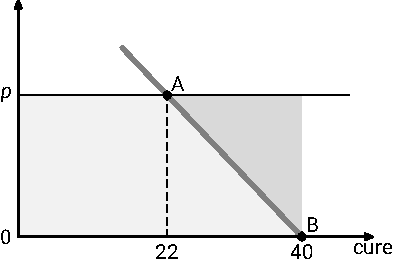
\includegraphics[height=4cm]{./figure/moral-hazard-2.pdf}
\end{figure}

\begin{itemize}
\item L'assicurazione rimborsa i costi dell'assistenza e azzera il prezzo al
momento dell'acquisto di cure: nell'esempio la quantità acquistata (40)
eccede il livello efficiente (22).
\item La perdita di benessere è data dal triangolo ombreggiato (differenza tra
costo e beneficio delle unità per le quali il primo supera il secondo)
\end{itemize}
\end{frame}


\begin{frame}{L'azzardo morale /2}
\begin{figure}[htbp]
\centering
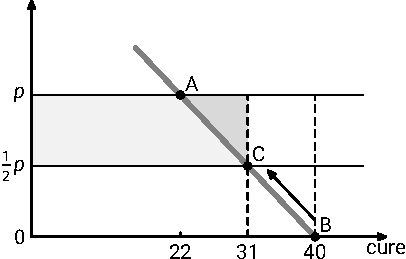
\includegraphics[height=4cm]{./figure/moral-hazard-3.pdf}
\end{figure}

\begin{itemize}
\item La soluzione ottimale non è la rinuncia ad assicurarsi, ma una riduzione
della copertura assicurativa
\item Ciò in quanto il rapporto tra perdita e beneficio dell'assicurazione aumenta
all'aumentare della percentuale di spesa rimborsata
\begin{itemize}
\item la risposta "di mercato" è l'adozione di forme di \emph{co-assicurazione},
copertura non completa delle spese sostenute
\end{itemize}
\end{itemize}
\end{frame}

\begin{frame}{L'azzardo morale: qual è la reale dimensione dell'inefficienza?}
\begin{columns}
\begin{column}{.5\columnwidth}
\small
\begin{itemize}
\item A: consumo in assenza di malattia (90 in beni di consumo)
\item B: consumo in presenza di malattia senza assicurazione (60 in beni di
consumo, 30 in cure sanitarie)
\item L'assicurazione costa 15 e azzera il costo delle cure. Con l'assicurazione
75 in beni di consumo, 66 in cure sanitarie)
\item Possiamo concludere che la spesa in eccesso è pari a 36? In realtà no!
\item Se invece di un rimborso della spesa l'individuo avesse ricevuto una
compensazione in somma fissa in grado di dargli la stessa utilità, la sua
spesa sanitaria sarebbe stata di 46 (punto D).
\end{itemize}
\end{column}

\begin{column}{.5\columnwidth}
\begin{figure}[htbp]
\centering
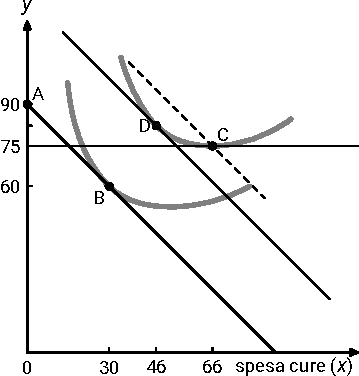
\includegraphics[height=5cm]{./figure/moral-hazard-effetto-reddito.pdf}
\end{figure}    
\small
\begin{itemize}
\item L'aumento da 30 a 46 non dipende dalla riduzione del prezzo, ma dal
maggiore reddito in caso di malattia: è un effetto di reddito che non comporta inefficienza!
\end{itemize}
\end{column}
\end{columns}
\end{frame}

\begin{frame}{L'azzardo morale e l'effetto reddito}
\begin{itemize}
\item L'aumento di domanda comporta un'inefficienza quando l'individuo, non
dovendo pagare le cure o pagandole meno del loro costo, alloca il suo
reddito alle cure anche quando il loro valore è inferiore a quello di
impieghi alternativi del reddito (\alert{effetto di sostituzione}).
\item Una parte dell'aumento di domanda può essere dovuto al fatto che
l'assicurazione aumenta il potere d'acquisto dell'individuo in caso di
malattia (\alert{effetto di reddito}). In questo caso non si ha inefficienza.
\item Un altro esempio: il sussidio di disoccupazione (Chetty, 2008)
\begin{itemize}
\item Il disoccupato può rifiutare un lavoro perché il costo di non lavorare è
più basso per effetto del sussidio (effetto distorsivo)
\item ma il rifiuto del lavoro può riflettere la volontà di cercare
un'opportunità migliore, più adeguata alle sue competenze, cosa che non
avrebbe potuto fare in assenza di sussidio (e con limitato accesso al
credito)
\end{itemize}
\end{itemize}

\begin{block}{}
APPROFONDIMENTO: per isolare l'effetto di sostituzione e individuare correttamente
la spesa in eccesso e la perdita di benessere è possibile utilizzare la \alert{curva di domanda compensata}.
\end{block}
\end{frame}

\section{La crescita della spesa sanitaria}

\begin{frame}{Evoluzione della spesa sanitaria}
\begin{figure}[htbp]
\centering
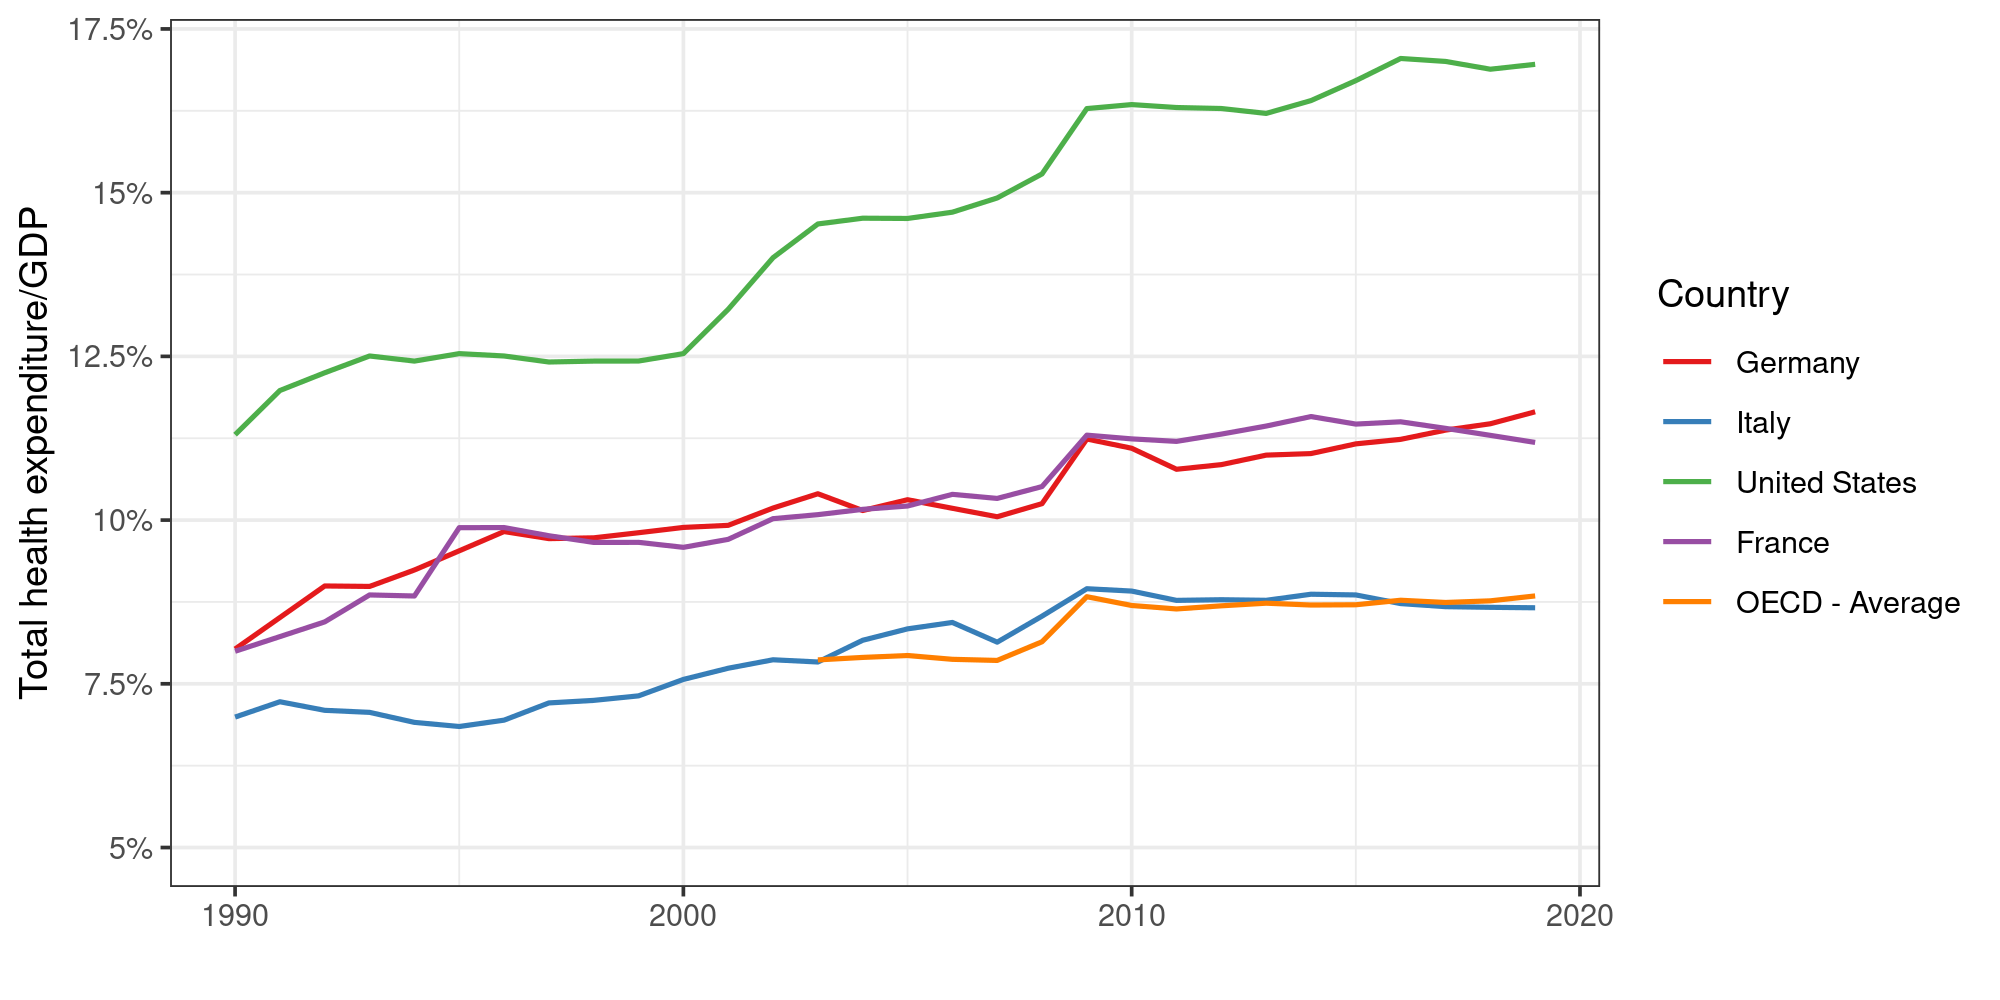
\includegraphics[height=5.5cm]{./figure/health-expenditure-growth-OECD.png}
\end{figure}
\vspace{-2mm}{\tiny
Fonte: OECD Health Expenditure and Financing \url{https://stats.oecd.org/Index.aspx?DataSetCode=SHA}
}

\begin{itemize}
\item La spesa sanitaria aumenta (molto) più velocemente del PIL
\end{itemize}
\end{frame}

\begin{frame}{Evoluzione della spesa sanitaria /2}
\begin{figure}[htbp]
\centering
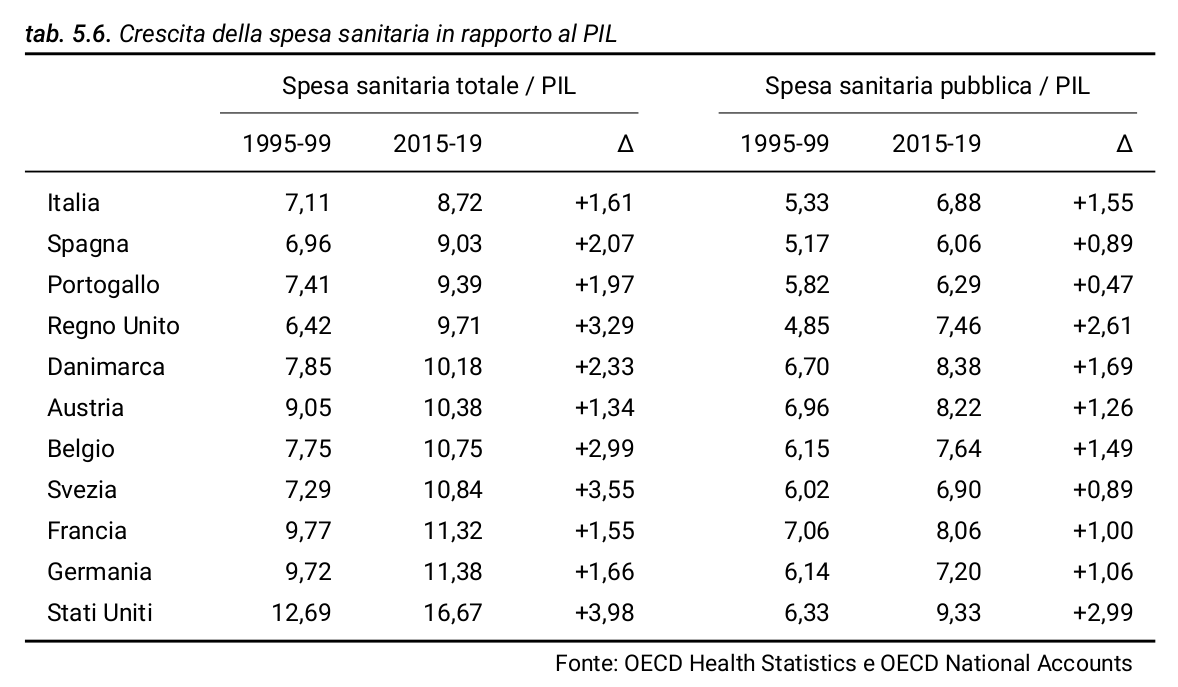
\includegraphics[height=6cm]{./figure/crescita-spesa-sanitaria.png}
\end{figure}
\end{frame}


\begin{frame}{Strategie di contenimento della spesa sanitaria}
\begin{description}
\item[{Sul lato domanda}] Partecipazione ai costi da parte dei pazienti
(co-assicurazione attraverso franchigie o coppertura parziale, ticket)
\begin{itemize}
\item L'efficacia dipende dall'elasticità della domanda, che nel caso della
sanità è piuttosto bassa
\item Scarsa efficacia se il paziente decide affidandosi al medico
\end{itemize}
\item[{Sul lato offerta}] Maggiore attenzione agli incentivi degli operatori
sanitari.
\begin{itemize}
\item Adozione di sistemi di pagamento prospettico invece che \emph{a piè di lista}
(negli USA: HMO e \emph{managed care})
\item \emph{Diagnosis-Related Groups} (DRG), utilizzati anche in Italia
(raggruppamenti omogenei diagnostici - ROD) per la spesa ospedaliera
\end{itemize}
Rischi: 
\begin{itemize}
\item segmentazione del mercato e scrematura
\item incentivi eccessivi al contenimento dei costi
\item "contabilità creativa" (nel caso dei DRG)
\end{itemize}
\end{description}
\end{frame}

\begin{frame}{Il contenimento della spesa}
\begin{itemize}
\item Il problema della deresponsabilizzazione della domanda è presente
sia nei sistemi pubblici che in quelli privati.
\item Nei sistemi centralizzati (pubblici) c'è più possibilità di controllo sulla
dinamica della spesa aggregata, attraverso la regolamentazione:
\begin{itemize}
\item tetti di spesa, vincoli alla crescita e espansione degli ospedali
\item accesso limitato a nuove tecnologie (controllo sugli investimenti)
\item riduzione delle quasi-rendite dei medici (minore remunerazione):
le remunerazioni reali dei medici sono cresciute del 35\% negli USA,
non sono cresciute negli altri paesi; negli USA i medici hanno
salario doppio (a fronte di reddito medio superiore solo del 10-20\%)
\item minor prezzo dei farmaci
\item riduzione nel livello di cure offerte e nel contenuto
tecnologico;
\end{itemize}
\item La maggiore spesa negli USA ha effetti limitati sulla salute:
presumibilmente il razionamento attuato dai sistemi pubblici riguarda cure
non essenziali
\end{itemize}
\end{frame}


\begin{frame}{Le cause della crescita della spesa}
\begin{itemize}
\item Possibili cause (fattori socio-economici):
\begin{itemize}
\item L'\alert{invecchiamento} spiega solo una piccola parte dell'aumento dei
costi. Aumenta il numero di anziani, ma migliora anche il loro stato di
salute.
\item L'\alert{aumento del reddito}: le stime USA danno un'elasticità della spesa al
reddito pari a 0.2-0.4 (ma le analisi \emph{cross-section} potrebbero
sovrastimare l'effetto per via del \emph{selection bias}). Se anche
l'elasticità fosse 1, spiegherebbe meno della metà della crescita.
\item L'\alert{estensione della copertura assicurativa} è un fattore una tantum.
\item Mutamenti nei comportamenti della popolazione (es. abitudini alimentari) o
dei medici (es. «medicina difensiva») non spiega abbastanza.
\item Effetto dell'aumento dell'offerta (domanda indotta dall'offerta): il
numero di medici aumentato meno della spesa, o non aumentato affatto).
\item L'aumento dei costi relativi («effetto Baumol»)
\end{itemize}
Nessuna di queste cause è considerata una spiegazione convincente.
\item La maggioranza degli studi individua quale fattore determinante
l'\alert{innovazione tecnologica}, che ha reso possibili nuove cure e
trattamenti. Ciò ha aumentato la domanda di cure.
\end{itemize}
\end{frame}

\begin{frame}{Dobbiamo preoccuparci della crescita della spesa?}
\begin{itemize}
\item Perché preoccuparci della crescita della spesa sanitaria? Non vale in
questo caso il principio della "sovranità del consumatore"?
\begin{itemize}
\item Il fatto che l'aumento sia così marcato si può spiegare con il fatto che la
salute è complementare a gran parte dei beni di consumo: acquistare salute
significa aumentare l'utilità del consumo di tutti gli altri beni.
\item D'altra parte, la scelta dei consumatori in questo caso può non
riflettere correttamente l'utilità, può essere falsata dalla presenza di
assicurazione e sussidi, oltre che da esternalità, razionalità limitata
ecc.
\item Ancora una volta il riferimento è alla presenza di \emph{azzardo morale}, al
fatto che i consumatori di cure non pagano per le spese sostenute al
momento del consumo.
\item Non solo inefficienza \emph{statica} (di cui abbiamo parlato). la distorsione
negli incentivi può condizionare l'intensità e tipo di innovazione
(\emph{inefficienza dinamica}): innovazione eccessiva e diretta verso trattamenti
eccessivamente costosi, non giustificati in termini di costi/benefici.
\end{itemize}
\item La crescita della spesa sanitaria è un problema per il bilancio pubblico.
\end{itemize}
\end{frame}
\end{document}